% !TeX program = xelatex
% Primary editable source. Initial body migrated from PR66 db086c7.
% Build from this directory with: tectonic 研究报告初稿.tex
% Competition-report layout follows the official 2026 template; the archived
% 2025 exemplars are used only as secondary references for content structure.
% Requires the existing figures/ directory. No Word conversion is used.
\documentclass[UTF8,a4paper,12pt,oneside,openany,fontset=fandol]{ctexrep}
\usepackage[
  top=20mm,
  bottom=20mm,
  left=20mm,
  right=20mm,
  headheight=15pt,
  headsep=5mm,
  footskip=10mm
]{geometry}
\usepackage{amsmath,amssymb,graphicx,longtable,tabularx,array,booktabs,alltt,needspace}
\usepackage[table]{xcolor}
\usepackage{fancyhdr}
\usepackage[font=small,labelfont=bf,labelsep=quad]{caption}
\usepackage[hidelinks,unicode,bookmarksnumbered]{hyperref}
\usepackage{xurl}
\newcommand{\reporttitle}{基于多类格困难假设的抗量子身份基匹配加密通用设计与优化实现}
\newcommand{\competitiontitle}{2026年第十一届全国密码技术竞赛作品设计报告}
\newcommand{\reportdate}{2026年10月20日}
% The competition platform assigns this value. Keep empty in review drafts and
% set it exactly once before running the submission-ready check.
\newcommand{\worknumber}{}
\newcommand{\worknumberfield}[1]{\underline{\makebox[#1][c]{\worknumber}}}
\hypersetup{
  pdftitle={\reporttitle},
  pdfsubject={\competitiontitle},
  pdfkeywords={身份基匹配加密, 格密码, HIBE, IBS, 抗量子密码}
}
\ctexset{
  chapter={format=\centering\heiti\zihao{2},beforeskip=0pt,afterskip=24pt},
  section={format=\heiti\zihao{3},beforeskip=18pt,afterskip=10pt},
  subsection={format=\heiti\zihao{4},beforeskip=12pt,afterskip=6pt}
}
\setlength{\parindent}{2em}
\setlength{\parskip}{0pt}
\linespread{1.28}
\setlength{\emergencystretch}{3em}
\setlength{\tabcolsep}{5pt}
\renewcommand{\arraystretch}{1.25}
\setlength{\LTpre}{9pt}
\setlength{\LTpost}{9pt}
\graphicspath{{figures/}}
\setcounter{tocdepth}{2}
\renewcommand{\listfigurename}{图目录}
\renewcommand{\listtablename}{表目录}
\newcommand{\reportheader}{全国密码技术竞赛作品设计报告}
\newcommand{\evidenceitem}[2]{\noindent #1\par{\noindent\scriptsize\color{black!70}\nolinkurl{#2}\par}\smallskip}
\fancypagestyle{frontmatter}{
  \fancyhf{}
  \renewcommand{\headrulewidth}{0pt}
  \renewcommand{\footrulewidth}{0pt}
  \fancyfoot[C]{\thepage}
}
\fancypagestyle{mainmatter}{
  \fancyhf{}
  \fancyhead[C]{\small\songti\reportheader}
  \fancyfoot[C]{\small\thepage}
  \renewcommand{\headrulewidth}{0.4pt}
  \renewcommand{\footrulewidth}{0pt}
}
\newlength{\tableavail}
\AddToHook{cmd/section/before}{\Needspace{8\baselineskip}}
\begin{document}
\hypersetup{pageanchor=false}
\pagenumbering{gobble}
\begin{titlepage}
\thispagestyle{empty}
\vspace*{7mm}
\noindent
\begin{minipage}[t]{0.73\textwidth}
\zihao{4}
作品编号：\worknumberfield{47mm}\\[8mm]
作品类别：\(\boxtimes\)软件设计\quad
\(\square\)硬件制作\quad
\(\square\)工程实践\\[3mm]
\hspace*{5em}\(\square\)密码应用技术\quad
\(\square\)其它
\end{minipage}%
\begin{minipage}[t]{0.27\textwidth}
\raggedleft

\includegraphics[width=30mm]{figures/cacr-logo.jpg}
\end{minipage}

\vspace{34mm}
\begin{center}
{\heiti\zihao{-2}\competitiontitle\par}
\vspace{5mm}
\rule{0.86\textwidth}{1.2pt}

\vspace{24mm}
{\zihao{3}作品题目：基于多类格困难假设的抗量子\par}
\vspace{4mm}
{\zihao{3}身份基匹配加密通用设计与优化实现\par}

\vfill
{\zihao{4}\reportdate\par}
\vspace{5mm}
{\zihao{4}中国密码学会\par}
\end{center}
\end{titlepage}

\clearpage
\thispagestyle{empty}
\begingroup
\zihao{-4}
\linespread{1.25}\selectfont
\setlength{\arrayrulewidth}{0.6pt}
\setlength{\tabcolsep}{3mm}
\renewcommand{\arraystretch}{1.18}
\noindent
\begin{tabularx}{\textwidth}{|>{\raggedright\arraybackslash}X|}
\hline
\centering\heiti\zihao{3}基本信息表\arraybackslash\\[1mm]
\hline
编号：\worknumberfield{48mm}\\
\hline
作品题目：\reporttitle\\
\hline
作品类别：\(\boxtimes\)软件设计\quad
\(\square\)硬件制作\quad
\(\square\)工程实践\quad
\(\square\)密码应用技术\quad
\(\square\)其它\\
\hline
\noindent\textbf{作品内容摘要：}\par
\setlength{\parindent}{2em}
身份基匹配加密要求通信双方同时满足身份条件。发送者指定接收身份，接收者指定期望的发送身份，只有双方身份均匹配时才能恢复消息。这一需求将消息保密与发送来源认证结合起来，但从论文构造走向可运行系统，还需要解决底层算法替换、参数独立配置、签名载荷容量、密文字节完整性和持久状态恢复等问题。

本作品采用 Wang 等提出的两层匿名分层身份基加密与身份基签名通用构造，建立 HIBE、IBS 与协议装配相互分离的软件框架。系统把接收身份置于 HIBE 第一层，把发送身份置于第二层，并使用 IBS 认证接收身份与消息。针对原语消息容量与应用载荷之间的差异，实现以32字节种子为入口的混合加密；针对原始密文表示可能存在的可修改空间，实现绑定完整内层密文字节的一次性签名包装。统一配置、规范序列化、固定发钥服务和状态加载机制用于支持多实例切换与新进程恢复。

本文冻结三组具有不同说明价值的完整系统。A 是可现场演示的工程基线，在3个独立根、9对热运行中，加密与解密中位数为0.211125和0.280116秒。B 保持同一LATTE HIBE，换用原生SRGG论文PARAM-I IBS；3个独立根、9对热运行的中位数为7.594920和0.201444秒。C 同时换用Lai C2 HIBE和Sageloli环SIS IBS，单根功能批次中一次加密为98.972055秒，一次诚实解密为424.980337秒，其中实际委派为393.037574秒。A、B、C的机器、线程及样本结构不同，这些数值逐组披露而不计算跨组加速比。

另对A完成同参数部署消融，将运行副本从 Windows 挂载目录移至 WSL 文件系统后，完整热加密与解密中位数由206.087和258.640毫秒降至10.921和56.360毫秒。该收益来自本机部署与文件访问开销，不能解释为格密码算法本身获得相同倍数的加速。

作品已形成命令行与网页演示，覆盖合法匹配、身份错配、密文修改和持久状态恢复。按已确认前提，已完成方案默认安全，HIBE具有身份匿名性，理论依据引用选定原文。三组精确配置的安装、恢复和有效外层下的内层签名拒绝均有实跑记录，A、B另有同机重复基准及最大消息边界。剩余工作为C的最大消息与有限重复、同发布版本复现及来源许可材料。
\\
\hline
\textbf{关键词（五个）：}身份基匹配加密；格密码；分层身份基加密；身份基签名；可复现评测\\
\hline
\end{tabularx}
\endgroup

\clearpage
\hypersetup{pageanchor=true}
\pagenumbering{roman}
\fancypagestyle{plain}{
  \fancyhf{}
  \renewcommand{\headrulewidth}{0pt}
  \renewcommand{\footrulewidth}{0pt}
  \fancyfoot[C]{\thepage}
}
\pagestyle{frontmatter}
\tableofcontents
\clearpage
\listoffigures
\clearpage
\listoftables
\clearpage
\pagenumbering{arabic}
\fancypagestyle{plain}{
  \fancyhf{}
  \fancyhead[C]{\small\songti\reportheader}
  \fancyfoot[C]{\small\thepage}
  \renewcommand{\headrulewidth}{0.4pt}
  \renewcommand{\footrulewidth}{0pt}
}
\pagestyle{mainmatter}
\chapter{作品概述}
\section{问题与应用场景}
考虑一个按身份投递保密消息的场景。发送者甲希望把消息交给身份为乙的接收者，乙希望只接收来自甲的消息。仅有接收者加密并不足以满足这一需求，因为能够生成密文不等于具有期望发送身份；仅有数字签名也不足以限制谁能读取消息。身份基匹配加密将两个条件放入一个协议，使解密同时依赖接收者持有的密钥身份和接收者给定的发送身份。[1]

本作品使用上述场景组织设计和演示。发送者在加密时使用自身签名密钥并指定接收身份，接收者在解密时使用自身接收密钥并指定期望发送身份。任何一侧不匹配，系统均应返回明确失败。这里的身份是协议使用的字节串；如何将邮箱、机构编号或自然人身份可信映射到该字节串，属于应用与发钥管理职责。原型未实现实名核验、开放注册或跨机构身份治理。

该原型用于展示算法和系统实现，不把演示场景写成已经落地的行业应用。它假定主密钥由可信发钥机构管理。发钥机构掌握主秘密，身份基体系固有的信任与密钥托管关系仍然存在，不能将系统描述为无信任第三方通信。

\section{自拟题目与验收对应}
仓库保存的2026年第十一届竞赛自拟题目要求模块化实现多类格方案，支持完整密钥生命周期、双向身份匹配、消息认证、密文完整性和统一评测。本稿按实际交付回答这些要求，而不把算法目录中的每条路线都当成已经可展示的完整系统。

\Needspace{8\baselineskip}
\begingroup
\small
\setlength{\tableavail}{\dimexpr\textwidth-4\tabcolsep\relax}
\begin{longtable}{@{}>{\raggedright\arraybackslash}p{0.25\tableavail}>{\raggedright\arraybackslash}p{0.35\tableavail}>{\raggedright\arraybackslash}p{0.4\tableavail}@{}}
\caption{自拟题目与已有成果对照}\label{tab:requirements}\\
\toprule
\rowcolor{black!8} 题目要求 & 已有实现与证据 & 本稿判断 \\
\midrule
\endfirsthead
\multicolumn{3}{l}{\small 表\thetable\quad 续表}\\
\toprule
\rowcolor{black!8} 题目要求 & 已有实现与证据 & 本稿判断 \\
\midrule
\endhead
\midrule
\multicolumn{3}{r}{\small 接下页}\\
\endfoot
\bottomrule
\endlastfoot
系统建立与双方发钥 & 统一 Setup、skgen、rkgen；三组完整收据 & 已有实际运行 \\
双向身份匹配 & 合法匹配及三类错配；Web与CLI验收 & 已有实际运行 \\
多类格路线的完整实例化 & LATTE＋ML-DSA、LATTE＋SRGG、Lai C2＋Sageloli环SIS均有完整运行 & 2种HIBE、3种IBS、3个冻结组合；见E15、E16 \\
非法身份与篡改拒绝 & IBS绑定、BYTEAUTH、严格解析及负向场景 & 已有功能证据；理论按引用与工作假设说明 \\
多方案切换 & 独立组件接口、配置、默认登记与预检 & 部分候选仅为单体后端 \\
时间尺寸内存与对比 & A、B重复基准，C目标规模单根运行；另有旧三组基线与部署消融 & 三代表已选定；不同环境数据不作等安全排名 \\
\end{longtable}
\endgroup
表中“完整实例化”包含实际调用对应原语及公共协议，不以 mock 或接口形状代替密码运算。“目标参数达标”则涉及实际版本、参数依据、容量和部署条件，需要单独结论。两个层次同时保留，便于评审判断项目已经实现什么、还欠缺什么。

\section{研究内容与作品贡献}
本作品首先实现可替换的 HIBE 与 IBS 接口，使两类原语分别配置参数，再由公共协议进行能力和容量检查。此设计避免把某个具体矩阵或陷门表示写入协议层，也使更换 IBS 时能够沿用相同的双向匹配流程。

其次，围绕论文算法之外的实际运行需求，实现规范对象编码、配置绑定、混合载荷、完整密文字节认证和固定发钥状态。这些机制使“同一身份重复使用”和“程序重启后继续使用”成为可验证的系统行为，而不只是一段内存中的诚实签验脚本。

再次，建立以完整系统为对象的评测材料，并针对实际热点进行受控优化。本文将原语采样、编码压缩、资源投影和完整系统部署实验分开讨论，避免用单体签名变小推断完整密文等比例变小，或用小维度运行推断目标规模已经可用。

通用构造、格原语、认证转换及底层签名库分别来自既有文献与实现。作品贡献集中于模块化实例化、工程机制、实现修订和可核查的实验分析，不宣称重新发明这些密码算法。

\section{报告范围}
本稿以普通隐私、加强认证、自我伪造防护和字节篡改拒绝为设计目标。Boyen-Li增强隐私及其 Ext、ReExt 操作不在实现范围。正文仅保留理解设计所需的格与原语概念，重点篇幅用于具体流程、参数、实现和实验。完整候选状态与证据位置放在附录，防止正文变成逐日开发记录。

\chapter{总体方案与安全依据}
\section{原语与角色}
分层身份基加密 HIBE 允许为身份路径生成密钥并向下委派。本文只需两层路径：父身份为接收者 r，子身份为发送者 s。接收者持有 r 的父级密钥，在指定期望发送者 s 后得到叶密钥。身份基签名 IBS 则允许使用主公钥和身份验证签名，发送者的签名密钥由机构按身份发放。[1-5]

LWE类问题提供带噪声线性关系的困难性基础，SIS类问题对应寻找满足模线性关系的短向量。环与模结构改变运算对象和实现成本。本文按每个实际后端记录其采用的假设与版本，不把 LWE、环LWE、模LWE、NTRU结构简单加总为互不相关的安全保证。困难假设、原语方案和完整组合采用不同计数口径。

系统包含可信发钥机构、发送者、接收者和可传输密文的信道。信道可以修改、截断或追加密文，因此解密过程必须先检查外层格式和认证，再恢复内部消息。实现层把预期密码学拒绝与运行异常分开报告，防止依赖缺失或后端崩溃被当成成功抵御攻击。

\begin{figure}[htbp]
\centering
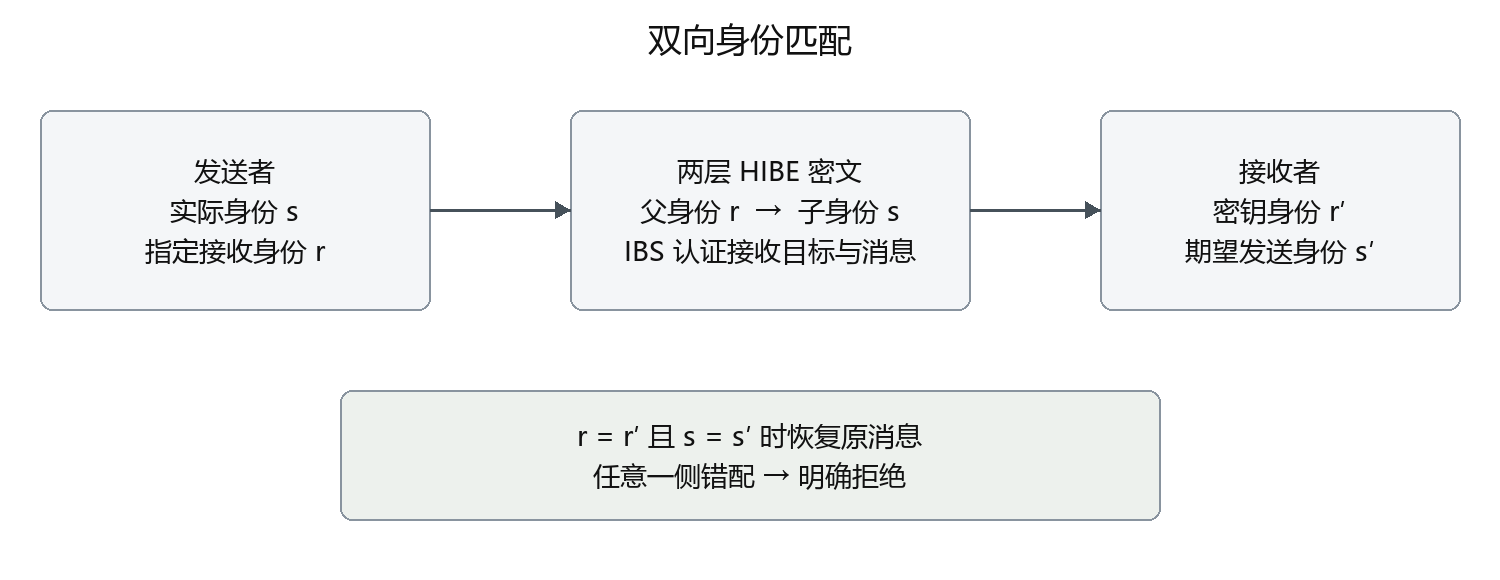
\includegraphics[width=\textwidth,height=0.52\textheight,keepaspectratio]{figures/matching.png}
\caption{身份双向匹配与两层路径}\label{fig:matching}
\end{figure}
图~\ref{fig:matching}中 s 是发送密钥绑定的实际身份，s\ensuremath{\prime}是接收者期望的发送身份；r 是加密目标，r\ensuremath{\prime}是接收密钥绑定的身份。诚实恢复条件为 s=s\ensuremath{\prime}且 r=r\ensuremath{\prime}。图示是正确性目标，拒绝效果仍由对应组合的实际试验验证。

\section{通用构造}
Wang等的通用构造将两层匿名HIBE与IBS组合。[1] 本项目基线流程与代码中的身份顺序一致，始终为 parent\_id=rcv、child\_id=phi，其中 phi 是发送密钥绑定的发送身份。令 Enc 表示带域分隔和长度前缀的规范编码，\ensuremath{\bot}表示密码学拒绝。

\Needspace{8\baselineskip}
\noindent\textbf{算法1 基线IBME流程}
\begingroup
\small
\setlength{\parskip}{0pt}
\begin{alltt}
Setup:
  (hpk, hmsk) \ensuremath{\leftarrow} HIBE.Setup(\ensuremath{\Pi\sb{H}})
  (ipk, imsk) \ensuremath{\leftarrow} IBS.Setup(\ensuremath{\Pi\sb{I}})
  mpk \ensuremath{\leftarrow} (hpk, ipk); msk \ensuremath{\leftarrow} (hmsk, imsk)
SenderKeyGen(msk, s):
  sks \ensuremath{\leftarrow} IBS.Extract(imsk, s)
ReceiverKeyGen(msk, r):
  dkr \ensuremath{\leftarrow} HIBE.Extract(hmsk, r)
Encrypt(mpk, sks, r, M):
  \ensuremath{\sigma} \ensuremath{\leftarrow} IBS.Sign(sks, Enc(r, M))
  P \ensuremath{\leftarrow} EncSignature(\ensuremath{\sigma}) || EncBytes(M)
  C \ensuremath{\leftarrow} HIBE.Encrypt(hpk, r, s, P)
Decrypt(mpk, dkr, s\ensuremath{\prime}, C):
  dkr,s\ensuremath{\prime} \ensuremath{\leftarrow} HIBE.Derive(dkr, s\ensuremath{\prime})
  P \ensuremath{\leftarrow} HIBE.Decrypt(dkr,s\ensuremath{\prime}, C)
  若解密、解析或签名加载失败则返回 \ensuremath{\bot}
  从P解析(\ensuremath{\sigma}, M)
  若 IBS.Verify(ipk, s\ensuremath{\prime}, Enc(r\ensuremath{\prime}, M), \ensuremath{\sigma}) 则返回M
  否则返回 \ensuremath{\bot}
\end{alltt}
\endgroup
签名输入包含接收身份，因此已经签发给某个接收者的消息不能直接作为面向另一接收身份的有效签名使用。HIBE路径与签名身份共同参与双向匹配。公共协议仅调用原语接口，不读取内部矩阵、采样陷门或私有多项式。

\section{混合加密与完整字节认证}
基线中HIBE需要承载签名与应用消息，而某些实际HIBE接口只适合承载短消息。项目的 Hybrid 层使 HIBE 只加密32字节随机种子，用 HKDF-SHA256 派生 AES-256-GCM 密钥承载完整内部载荷。配置中同时保留种子长度、原始身份长度、内层身份编码长度和载荷上限，避免把32字节种子误写为只能发送32字节应用消息。当前展示配置的原始身份上限64字节，内层对应86字节。[E01-E04]

BYTEAUTH层使用新生成的 Lamport 一次性签名密钥认证完整内部密文字节，并绑定公共上下文。一次性公钥的承诺被放入由IBS签名覆盖的内部消息中；解密后还要比较内部承诺与外层一次性公钥。这个内外绑定步骤用于防止攻击者仅替换外层一次性公钥并重新签名，就把已有内部密文包装成新的有效发送内容。

完整解密依次检查规范格式、公共上下文和一次性签名，再调用内部IBME恢复，最后核对承诺并输出原始应用消息。不同层的认证职责不能相互替代：GCM检查混合载荷，IBS认证发送身份及接收目标，BYTEAUTH覆盖完整内部密文字节。它们也都不能由“测试全部通过”推导出新的CCA或QROM定理。

\begin{figure}[htbp]
\centering
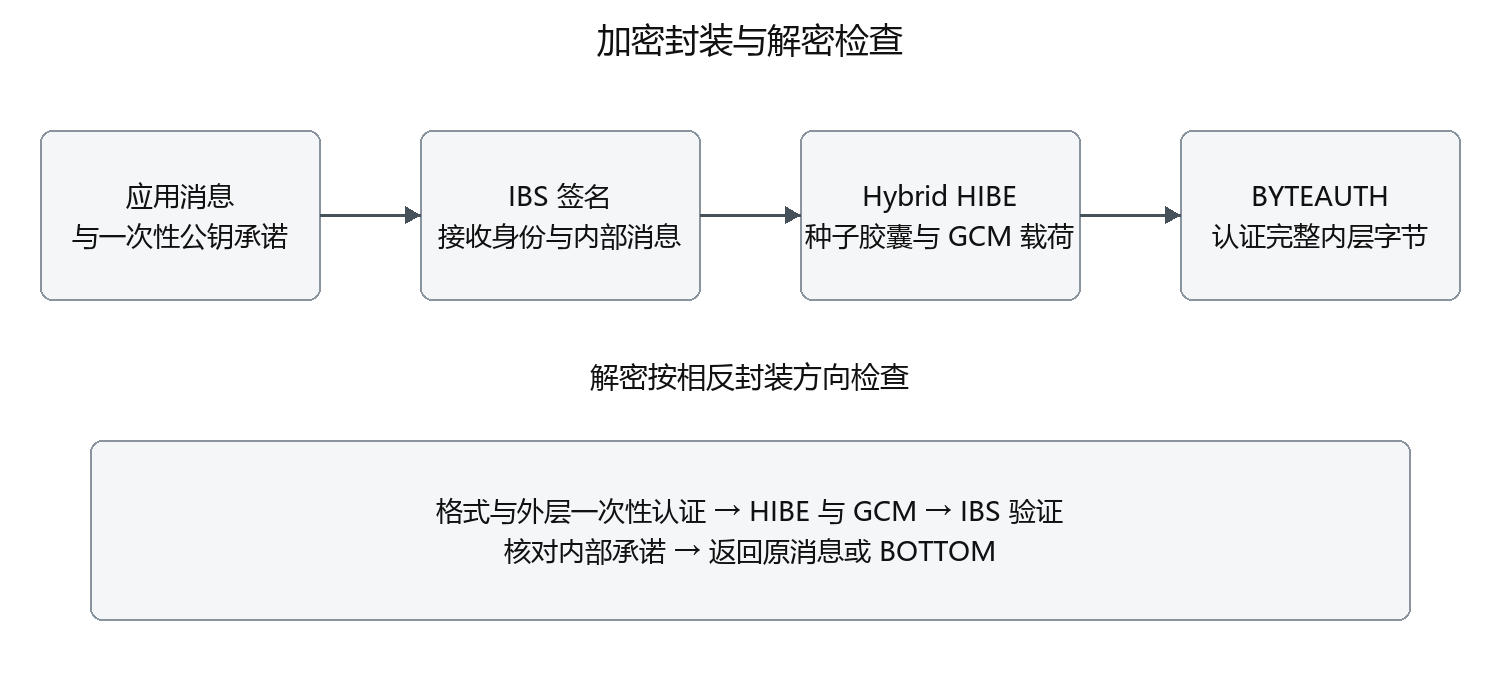
\includegraphics[width=\textwidth,height=0.52\textheight,keepaspectratio]{figures/layers.png}
\caption{加密封装与解密检查顺序}\label{fig:layers}
\end{figure}
\section{理论引用与项目工作前提}
理论部分以固定版本原文为依据。Wang通用构造、CHKP、Luo及认证转换分别按相应文献引用；ML-DSA采用FIPS204中的算法版本，Falcon采用归档的v1.2规范与固定实现。[1-5,11-13] 引用底层标准只说明底层普通签名的来源，不意味着认证转换后的IBS或整个IBME获得相同标准认证。

项目于2026年10月18日确认工程前提：按所选论文算法具备所需安全性、HIBE具有身份匿名性继续研发。原文已明确给出的性质作为引用，未明确给出的部分标明工作假设。例如本稿不把LATTE的普通机密性结论直接改写为已在本项目证明的身份匿名性。该区分用于说明设计依据，不另设基础证明工程作为实现前置任务。

实际参数、采样与已知失败仍如实报告。2026年10月20日明确采用“已完成方案默认安全”的前提，完成并冻结采用的精确profile使用security\_claim=secure、backend\_admitted=true、parameters\_are\_formal=true；A、B、C均在该范围内。安全目标与模型分别引用原文，该前提不等同于完整 IB-ME 获得外部 NIST 认证。mock、教学档、已知公开攻击负控、仅数值投影和未完成后端继续单列。[E17]

\chapter{多算法实例化与参数选择}
\begingroup
\linespread{1.05}\selectfont
\section{独立配置与筛选方法}
统一框架分别保存HIBE参数、IBS参数、签名编码、传输方式和状态策略。装配时先检查接口能力和输入容量，再决定是否允许运行。配置可被解析只代表配置格式合法；单体可运行、默认可选、已完成实际配对和取得重复性能收据是不同状态。

候选选择同时考虑原文与实现版本能否对应、是否具有真实采样与签验链、输入容量能否容纳封装后的签名消息、是否支持规范保存和恢复，以及本机可承担的时间和内存。某个算法的高维目标难以运行时，仍保留其资源研究价值，但不能用小维度实验补足目标运行数量。

截至本稿更新，公共registry已经登记LATTE、Lai、ABB-ROM、CHKP及明确命名的MP12变体，并登记Luo、SRGG默认档与论文档、Sageloli环v3、认证转换型ML-DSA/Falcon及Wang-PW等IBS。登记、运行时可用、精确profile准入和完整组合实跑分别记录；不能用其中一列替代其它列。附录A按19条论文路线列出当前状态。

\section{冻结的三组报告代表}
三组均使用Hybrid、BYTEAUTH和单写者状态策略，但不再只更换IBS：A、B共享LATTE-3/COSAC-FIX，C使用Lai C2。外部身份上限均为64字节，Hybrid内层身份为86字节，底层HIBE只加密32字节种子。载荷预算是内部协议预算，不等于应用消息容量。[E15]

\begingroup
\small
\setlength{\tableavail}{\dimexpr\textwidth-6\tabcolsep\relax}
\begin{longtable}{@{}>{\raggedright\arraybackslash}p{0.24\tableavail}>{\raggedright\arraybackslash}p{0.27\tableavail}>{\raggedright\arraybackslash}p{0.25\tableavail}>{\raggedright\arraybackslash}p{0.24\tableavail}@{}}
\caption{展示配置与用途}\label{tab:representatives}\\
\toprule
\rowcolor{black!8} 代表 & 精确组合 & 主要用途 & 容量与边界 \\
\midrule
\endfirsthead
\multicolumn{4}{l}{\small 表\thetable\quad 续表}\\
\toprule
\rowcolor{black!8} 代表 & 精确组合 & 主要用途 & 容量与边界 \\
\midrule
\endhead
\midrule
\multicolumn{4}{r}{\small 接下页}\\
\endfoot
\bottomrule
\endlastfoot
A & LATTE-3＋BNN/ML-DSA-44 reference & 主演示、安装与恢复基线 & 64KiB载荷预算；应用消息上限59191B \\
B & LATTE-3＋SRGG PARAM-I compact & 原生模块格IBS与无损编码 & 128KiB载荷预算；应用消息上限65364B \\
C & Lai C2＋Sageloli RSIS v3 PARAM-I & 另一HIBE与原生环IBS目标规模 & 8MiB载荷预算；应用消息上限3924B；分钟级解密 \\
\end{longtable}
\endgroup
A、B的LATTE参数为N=1024、q=68718428161、seed32模式，最多2个接收父身份、每父2个发送子身份。A的认证转换签名包含用户公钥、机构证书与消息签名，不能用底层ML-DSA单个签名大小代替完整IBS尺寸。[4,11,12]

B采用SRGG论文PARAM-I，基础参数为n=512、rank=2、p=16383、base=31、digits=2。实现同时冻结Q=15744063、factor1和表格标准差解释。原文标称目标100 bit，并列出量子密钥恢复／伪造95／93 bit；这里只引用作者口径，不把它改写为完整IBME的统一安全等级。[6,E15]

C采用Lai C2的n=2048、q=274877976577、k=39、l=2，与Sageloli PARAM-I的d=2048、k=65、l=132、q=\(3^{65}\)组合。该配置真实完成目标规模完整运行，但密钥、密文和委派成本高，定位是结构覆盖与资源边界而非性能冠军。[10,15,E16]

三组的选择依据是已有完整运行、参数与源码可追溯、避开已知攻击调试档，并分别提供主演示、原生IBS和另一HIBE的解释价值。安全目标、机器与样本边界不同，因此本文逐组报告，不计算“最安全且最快”的总排名。旧ML-DSA／Falcon／Luo三组重复基线继续作为辅助对照，不再占用最终代表名额。

\section{原生IBS的已完成范围}
Luo矩阵版与模格版均有研究实现。模格版是当前Luo工程主线，已完成规范对象、签名编码、固定身份服务及真实组合。显式C64B变体调整\(\gamma_1\)、\(\gamma_2\)、\(\gamma_3\)与重试上限，已有LATTE完整基准；它仍是同一种IBS的参数变体，不新增算法数量。其应用消息容量上限3924字节与IBS输入4096字节分开记录。[E05]

Wang基本IBS加Pan-Wagner转换已经具有真实MP12采样、身份盐和消息盐、完整签验以及保存恢复链，默认入口已有LATTE实际配对记录。[1,7,E06] 当前已配对的q17调试配置具有公开伪造问题，不能作为安全主展示参数。完整实现与安全参数可用是两项独立结论。

SRGG已经形成完整研究IBS及论文参数三档独立运行。其工作包括相关扰动采样、Schur部分处理、原像生成、挑战与完整签验。compact编码不改变原签名对象，可对公钥、主秘密、身份密钥与签名进行无损存储压缩。论文参数路线现已作为\texttt{srgg2025-paper}登记，PARAM-I compact与LATTE组成代表B，并有精确128KiB Suite的34项功能检查和三根重复基准；默认小参数路线的旧结果仍不自动继承。[6,E07,E15]

Foo-Li、Yu2026与Sageloli-SIS、Sageloli-RSIS已有完整单体研究后端。其中Sageloli实现覆盖H1/H2、盐、矩阵或环上的采样与签验、固定发钥及恢复；环版v3已作为\texttt{sageloli-rsis}登记，论文PARAM-I／II获默认安全口径。PARAM-I先与LATTE完成安装恢复桥接，再与Lai C2组成代表C并完成真实完整运行。[E14,E16] Yu当前实现的消息容量仅1至4字节，无法容纳公共构造实际签名输入，预检应拒绝该组合。Xie-NTRU路线已有修订研究核，但还不是共同IBSBackend。本文不把组件、数学探针或取得的通用NTRU工具计算为完整IBS。[8-10,E08]

\section{HIBE资源研究与目标规模}
CHKP研究实现需要明确原稿版本。项目现有3m叶布局与出版版2m比较对象不同，不能把两种布局的参数与定理混用。高基数MP12结构化种子KEM组件已完成根、父、256个叶和32字节种子路径；相关研究变体已有明确命名的公共后端，但目标参数完整运行仍未交付，不能把小参数接线当作出版版目标。[2,14,E09]

已有n=2、4、8且q约93比特的有界运行，用于验证算术、委派、编码和恢复。n=8的父生成约4.15秒、256叶约44.78秒、观测RSS约225MiB。目标n=4096未生成密钥；资源投影中的父陷门约9GiB、探测载荷约19.197GiB均为模型估算，不是测量结果。更大机器或不同表示可能改变可部署性，因此不能从当前环境限制推出算法普遍不可行。

ABB最新紧边界候选n=8224、模数约180比特、噪声参数721，公开模型给出的完整基表示字节下界为473331337067574字节，32字节原始密文为52296768512字节。该批只做公开算术与成本比较，尚无目标密钥和完整运行。估计器中根SIS没有有限估计值，含义为该模型未给出有限成本，不能写作“无限安全”。[3,E10]

这些研究说明参数选择与表示成本会直接影响完整组合。它们可作为未选路线的资源证据，却不能覆盖已冻结的A、B、C，也不能把仅有投影的候选写成已经实现、运行或已被淘汰的最终方案。

\section{原生IBS参数研究与目标规模（Foo-Li）}
Foo-Li后端已具备五方法、固定发钥与恢复的完整单体实现，但本稿按E13已核对的ACISP会议版与作者机构开放版记录使用论文的渐近充分条件，未据此宣称已检索所有可能的扩展稿；所核对版本未给出可直接复用的数值实例，与Sageloli论文列出两组数值点的方式不同。[8,E13] 因此该路线的具体参数只能由实现方从论文充分条件推导。当前可运行的q=3、n=1教学配置存在公开伪造，不能作为参数代表。

本作品对该路线做了两层参数工作。第一层是有限网格预筛：在后端参数门的选定网格内（素数位长3至32每档最大素数、n至4、生成宽度16至\(2^{28}\)九档）检查正则性与质量链联动，621个探针未找到可交精确筛查的候选窗口；预筛使用浮点镜像并带四比特余量，空窗口不是严格排除证书，也不覆盖网格外的合法形状，因此只表述为该网格内未发现，而非全部门内参数的否定。第二层是目标推导：在门外的q至2\textasciicircum{}127\ensuremath{-}1、n至4096范围内做带失败归因的搜索，240个候选中130个未通过解析检查、64个被标准LLL界排除、44个经典硬度估计不足，其余2个通过当前解析模型检查且经典core-SVP估计不低于128比特。该方案质量链使归约范数快速增长，本批已测经典128比特估计点位于n=4096，如表~\ref{tab:fooli-grid}所示。

\begingroup
\small
\setlength{\tableavail}{\dimexpr\textwidth-6\tabcolsep\relax}
\begin{longtable}{@{}>{\raggedright\arraybackslash}p{0.24\tableavail}>{\raggedright\arraybackslash}p{0.27\tableavail}>{\raggedright\arraybackslash}p{0.25\tableavail}>{\raggedright\arraybackslash}p{0.24\tableavail}@{}}
\caption{Foo-Li选定网格的core-SVP估计（\(q=2^{127}-1\)、g=16，各n取本批最小\ensuremath{\bar m}，Chen-Nguyen启发式）}\label{tab:fooli-grid}\\
\toprule
\rowcolor{black!8} n & 完整维度d & 经典／量子（比特） & 本模型判断 \\
\midrule
\endfirsthead
\multicolumn{4}{l}{\small 表\thetable\quad 续表}\\
\toprule
\rowcolor{black!8} n & 完整维度d & 经典／量子（比特） & 本模型判断 \\
\midrule
\endhead
\midrule
\multicolumn{4}{r}{\small 接下页}\\
\endfoot
\bottomrule
\endlastfoot
1024 & 390,160 & 15.2／13.8 & 搜索下限 \\
2048 & 780,304 & 51.4／46.6 & 经典估计不足128 \\
4096 & 1,560,592 & 129.9／117.9 & 仅经典估计不低于128 \\
\end{longtable}
\endgroup
表~\ref{tab:fooli-grid}每行完整参数和\ensuremath{\bar m}在report-facts.json中绑定E13逐点记录，维度满足d=\ensuremath{\bar m}+2nk。n=1024的15.2／13.8来自b=53搜索下限；搜索下限不表示已求出实际最便宜攻击，也不能据本批网格证明4096是所有参数域的最小可行维度。

按E13公钥估计排序的最小候选为\(q=2^{127}-1\)、n=4096、\ensuremath{\bar m}=520208，公钥紧凑比特打包估计约63GiB，经典core-SVP估计129.94、量子117.93比特；本批没有同时达到经典与量子128的候选。该候选未生成目标密钥，且超过现后端执行门。其余主密钥、用户私钥和签名的目标尺寸需在明确表示和计算公式下另行核算，不作为本稿已测数据。

作为资源示例，E14的Sageloli环版PARAM-I公钥序列化实测约3.35MiB、发钥约85秒、新建进程峰值约1.36GiB；Foo-Li上述约63GiB则是尚未运行候选的公钥打包估计。两种方案的安全模型、参数和统计口径不同，不能把这两个点写成同安全级性能排名或整条路线的固有代价，也不以本机内存判断算法不可行。core-SVP是启发式估计；Sageloli PARAM-I当前为默认安全口径profile，Foo-Li未运行候选仍为none/false/false。

\par\endgroup
\chapter{系统实现与关键技术}
\section{分层架构与公共契约}
系统由原语层、协议装配层、状态与传输层、应用入口和评测工具组成。HIBE后端负责建立、父密钥提取、向下委派、加密、解密和对象加载；IBS后端负责建立、身份密钥提取、签名、验证和签名加载。规范对象提供序列化与明确的上下文检查。协议层通过这些契约组合原语，不依赖某一种内部矩阵维度。

\begin{figure}[htbp]
\centering
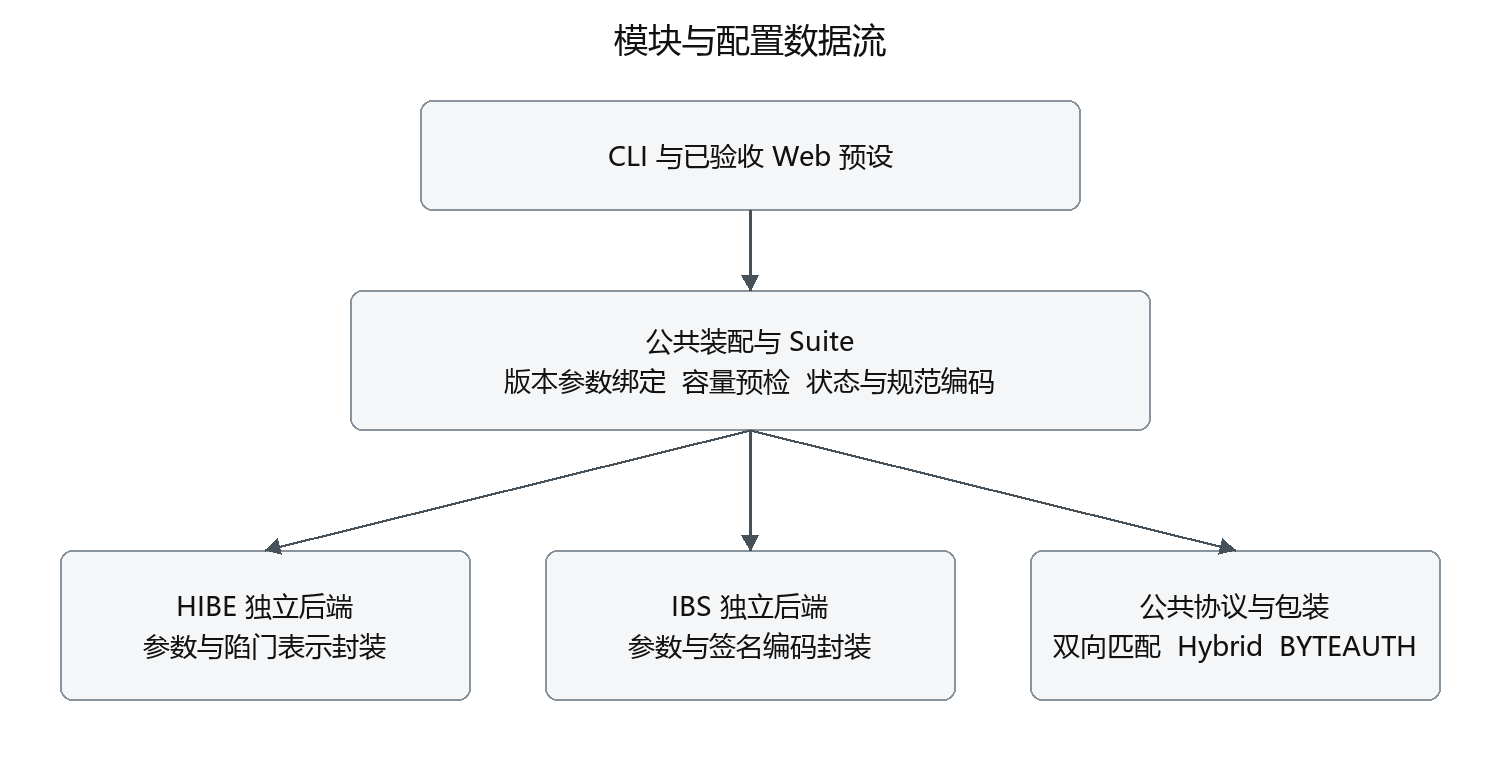
\includegraphics[width=0.88\textwidth,height=0.52\textheight,keepaspectratio]{figures/architecture.png}
\caption{软件模块与配置数据流}\label{fig:architecture}
\end{figure}
公共Suite绑定算法版本、两组原语参数、签名格式、包装及状态策略。相同的算法名称但不同参数、编码或上下文不能静默混用。装配预检还要计入身份编码和BYTEAUTH内部承诺产生的额外字节，发现容量不足时在发起长计算前明确拒绝。

新算法在自身registration模块提供显式provider，返回完整BackendSpec；调用方可在独立registry中原子加入一个或一组HIBE／IBS描述符，不必复制协议或修改中央注册表。任一描述符不完整或ID重复时整批拒绝，不留下半注册状态。Suite JSON只能选择已经登记的ID，不能携带Python导入路径；CLI的签名格式也由所选IBS描述符校验，而不是维护固定算法白名单。

源码中的研究后端不会因为实现了接口就自动出现在网页预设中。网页当前公开LATTE＋ML-DSA／Falcon／Luo三个交互预设，其中只有ML-DSA对应代表A；报告代表B、C因运行时间和资源边界通过CLI、冻结Suite及预运行收据展示。此设计避免分钟级组合阻塞现场页面，也防止把Web集合误写成最终三代表。

\section{规范编码与错误处理}
身份、消息和签名使用域分隔及长度前缀编码。解码器验证对象种类、版本、字段数量、尺寸上限和规范表示，并拒绝截断、追加及重复字段。模q系数、向量维度和环参数由对应后端检查，不能仅凭能够反序列化便进入密码运算。

密码学拒绝使用专用BOTTOM值，不能把Python的None、任意空对象或后端异常当成同一结果。验收中，合法解密必须逐字节等于原消息；负向场景必须得到预期拒绝。执行失败单独报告。这样的判定避免“程序没有得到明文”被误记成安全机制正确工作。

字节认证测试针对实际完整wire执行。测试范围包含单字节修改、签名修改、截断、追加和重复字段。底层CPA解密对某些扰动的容错与外层严格字节认证承担不同职责，不能要求原始CPA算法单独提供本不具备的完整字节唯一性。

\section{固定发钥缓存与持久恢复}
系统按身份维护已发放密钥与必要委派状态。相同身份的再次请求使用同一服务语义，不能在恢复时重新抽取密钥以掩盖丢失。状态更新采用单写者、提交后发布的策略，失败或未完成操作不能伪装成已发放状态。某些论文实验中的每次重新提取与本项目长期服务语义存在区别，相关适配保留在原语说明中。

持久化内容按公开状态、主秘密、发送状态和接收状态分开核对。新进程加载阶段在零熵条件下复原已有对象，以检查加载没有重新执行Setup、发钥或秘密采样。后续新加密和新签名仍使用新CSPRNG；“零熵恢复”不意味着正常密码操作不需要随机数。

运行秘密、主私钥及原始私有状态不进入公开Git材料。公开实验只保留参数、时间、尺寸、公开钥指纹、源码指纹和检查收据。compact编码只压缩表示，不加密秘密快照，因此不能把密钥文件变小解释为密钥已经获得存储保密保护。

\section{原语实现与编码优化}
原语实现保持论文步骤与工程修订可区分。例如Wang-PW把基本IBS与转换链分别实现，不能只加两个随机盐就称转换完成；Sageloli保留矩阵与环路线各自的采样对象；SRGG在独立路线中明确高斯参数解释，不将实现选择表述为作者已经发布勘误。[6-10]

SRGG最新编码根据系数范围采用24比特公系数、2比特CBD1陷门分量、整数Zigzag及1比特挑战表示，解码后重建原对象。压缩前后应保持公钥、签名、验证方程和上下文一致，编码与恢复阶段不额外抽取随机数。它解决的是公开传输与落盘表示冗余，完整操作可能因编码开销变慢，RSS也不会按文件压缩比例下降。[E07]

高基数陷门工具则研究大模数下gadget位数与委派表示的代价。该工具及种子KEM组件的效果在自身实验范围内描述，未接入完整系统前，不给出IBME加速结论。

\section{原生依赖核对与部署优化}
LATTE及认证型签名适配器调用原生程序，运行前核对固定源码、ABI与二进制。剖析发现Windows挂载目录上的频繁读取与哈希占据明显时间。本项目保持这些校验，构建按wheel内容SHA定位的WSL运行副本，使已打包内容从WSL文件系统读取。[E11]

运行副本在安装及复用时核对内容文件和元数据，检查包成员路径与额外Python提供者。原生程序仍使用同一构建，不复制运行私钥或修改全局Python环境。仓库代码更新后需要重新构建并指定新wheel，已有副本不会自动切换。安装、导入和恢复开销独立于热操作计时，不能把这些启动成本隐去后宣称所有场景都获得同样收益。

\chapter{实验设计结果与分析}
\section{数据来源与实验问题}
本章整理仓库已经归档的实验，不为撰稿重新生成密钥，也不把本次文档生成计为新的密码学试验。每张表对应固定公开JSON与源码版本。实验回答四个问题：冻结组合是否完成匹配与拒绝；A、B重复运行及C目标规模运行的实际成本是多少；完整wire和状态尺寸处于什么量级；部署位置改动能否在相同密码工作下减少完整操作耗时。

A使用Intel Core Ultra9 275HX、Sage10.9／Python3.13.14、OMP4／BLAS1；B使用i9-14900HX、Sage10.7／Python3.12.13、OMP4／BLAS1。二者均为3套独立CSPRNG系统状态、9对热运行和9次恢复后解密。C使用Ultra9 275HX、Sage10.9／Python3.13.14、OMP1／BLAS1，四个IBS组合共享1个Lai根与2个一级钥；所选C只有1次加密和每种身份情形1次解密。三组均使用64字节外部身份和32字节应用消息。[E15,E16]

冷状态指新的Python进程，保留操作系统页缓存和已构建原生程序，不是断电或清空所有缓存后的启动。热运行复用各自状态，不把9次观察当成9套独立密钥。10毫秒进程树RSS可能漏掉短峰或重复计共享页；C还分别记录准备阶段进程树采样和解密进程内核生命周期高水位。不同口径不拼接成统一排名。

\section{功能拒绝与恢复}
\begingroup
\small
\setlength{\tableavail}{\dimexpr\textwidth-4\tabcolsep\relax}
\begin{longtable}{@{}>{\raggedright\arraybackslash}p{0.25\tableavail}>{\raggedright\arraybackslash}p{0.35\tableavail}>{\raggedright\arraybackslash}p{0.4\tableavail}@{}}
\caption{完整系统功能证据}\label{tab:functional-evidence}\\
\toprule
\rowcolor{black!8} 场景 & 期望结果 & 已有证据 \\
\midrule
\endfirsthead
\multicolumn{3}{l}{\small 表\thetable\quad 续表}\\
\toprule
\rowcolor{black!8} 场景 & 期望结果 & 已有证据 \\
\midrule
\endhead
\midrule
\multicolumn{3}{r}{\small 接下页}\\
\endfoot
\bottomrule
\endlastfoot
发送与接收均匹配 & 原消息逐字节恢复 & A的Web／安装CLI，B的34项功能矩阵，C的真实完整解密 \\
仅发送身份错配 & BOTTOM & A的Web／CLI，B功能矩阵，C实际委派后拒绝 \\
仅接收身份错配 & BOTTOM & 同上 \\
双方身份错配 & BOTTOM & 同上 \\
修改截断追加或重复密文 & 解析失败或密码学拒绝 & 三组精确安装wire验收及有效外层下的内层签名负例[E18] \\
固定状态加载与再次解密 & 不重新发放既有身份钥且消息一致 & A、B各9次恢复解密；三组精确CLI恢复，C实际重新委派[E18] \\
服务异常 & 明确执行失败 & 不纳入拒绝成功统计 \\
\end{longtable}
\endgroup
网页的LATTE＋ML-DSA／Falcon／Luo三个辅助预设已有18项核心场景。网页刷新可以重连临时会话，但服务重启会丢失网页会话，持久恢复由CLI状态路径提供。E18已逐组实测B的128KiB安装、C的精确安装恢复和有效外层下的内层签名拒绝。A、B恢复零新熵；C没有叶缓存，每次恢复解密实际重新随机委派。[E12,E15,E18]

\section{三代表完整运行观察}
\begingroup
\small
\setlength{\tableavail}{\dimexpr\textwidth-6\tabcolsep\relax}
\begin{longtable}{@{}>{\raggedright\arraybackslash}p{0.22\tableavail}>{\raggedright\arraybackslash}p{0.28\tableavail}>{\raggedright\arraybackslash}p{0.25\tableavail}>{\raggedright\arraybackslash}p{0.25\tableavail}@{}}
\caption{冻结三代表的完整协议观测}\label{tab:representative-observations}\\
\toprule
\rowcolor{black!8} 代表 & 样本边界 & 完整加密／解密（秒） & 完整密文wire（字节） \\
\midrule
\endfirsthead
\multicolumn{4}{l}{\small 表\thetable\quad 续表}\\
\toprule
\rowcolor{black!8} 代表 & 样本边界 & 完整加密／解密（秒） & 完整密文wire（字节） \\
\midrule
\endhead
\midrule
\multicolumn{4}{r}{\small 接下页}\\
\endfoot
\bottomrule
\endlastfoot
A & 3根、9对热运行；中位数 & 0.211125／0.280116 & 142051--142146 \\
B & 3根、9对热运行；中位数 & 7.594920／0.201444 & 149191--149291 \\
C & 1个共享HIBE根；单次观察 & 98.972055／424.980337 & 4555436 \\
\end{longtable}
\endgroup
表~\ref{tab:representative-observations}只把三组放在同一位置说明量级，不构成统一统计比较。A与B的数值是热运行中位数，C是一次目标规模观察且解密包含393.037574秒的真实Lai委派；A、B、C的机器和线程设置也不同。C的结构覆盖价值不能改写为性能优势，A、B的中位数也不能与C单次值计算加速比。

后续同机补充批次E18在同一源码wheel、i9-14900HX、Sage10.7／Python3.12.13、OMP4／BLAS1下顺序运行A、B，各3个独立根、9对热运行及9次恢复解密。结果见附录表~\ref{tab:same-machine-ab}；该批次与表~\ref{tab:representative-observations}的原始收据分别记账，不拼接成更大样本。A、B的实际参数目标仍不同，同机条件也不构成等安全排名。

\begin{figure}[htbp]
\centering
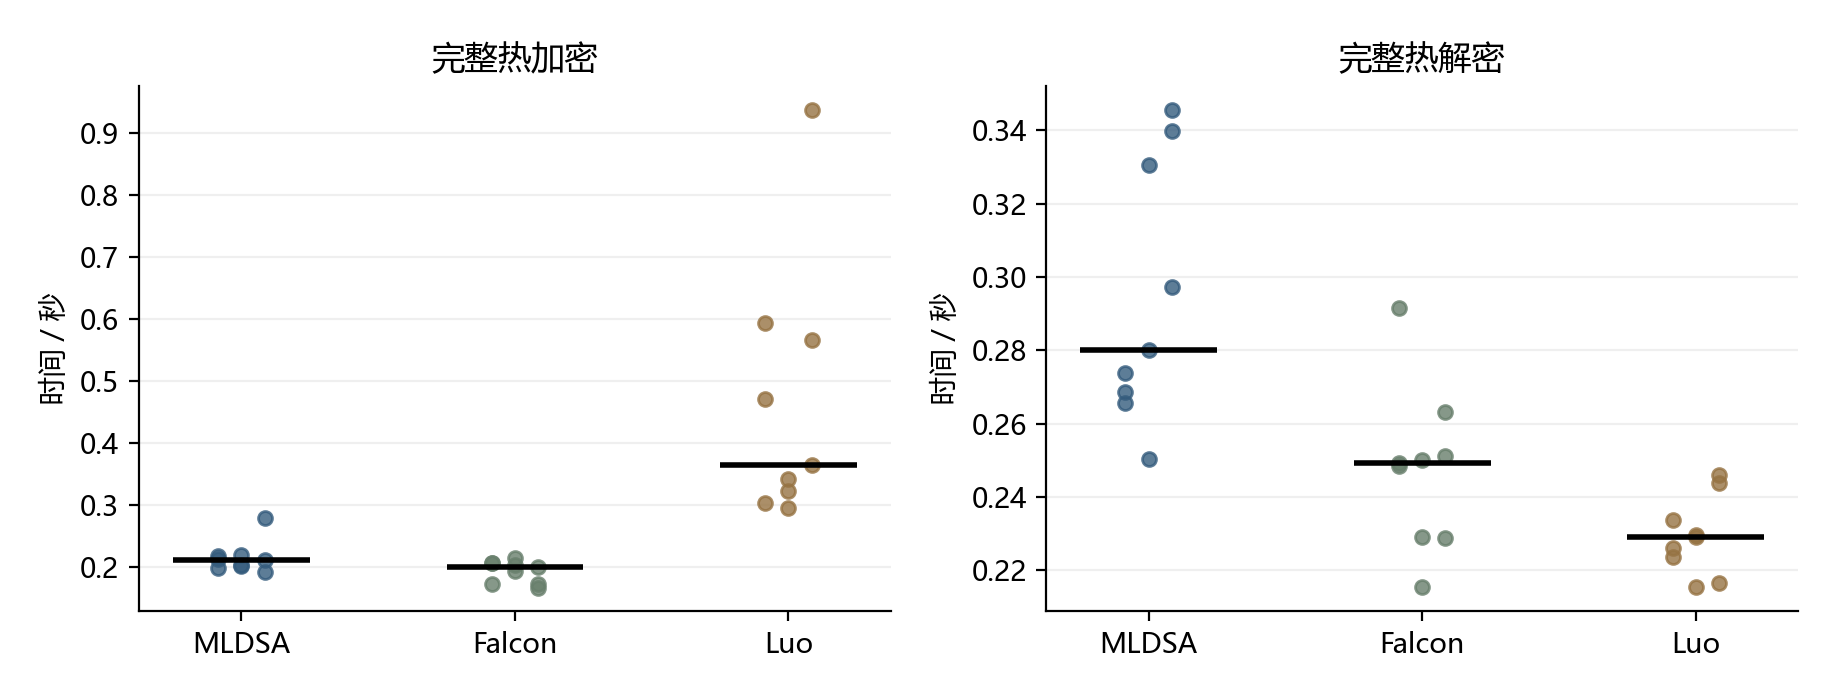
\includegraphics[width=\textwidth,height=0.52\textheight,keepaspectratio]{figures/baseline.png}
\caption{旧LATTE三IBS辅助基线的热运行观察}\label{fig:legacy-baseline}
\end{figure}
图~\ref{fig:legacy-baseline}保留ML-DSA、Falcon和Luo三组旧辅助基线的9次热运行观察，并以短横线表示中位数。它用于分析固定LATTE下的工程差异，不代表新的A、B、C，也不能用于宣称低概率失败界或大规模用户吞吐保证。

\section{完整尺寸与内存}
\begingroup
\small
\setlength{\tableavail}{\dimexpr\textwidth-6\tabcolsep\relax}
\begin{longtable}{@{}>{\raggedright\arraybackslash}p{0.34\tableavail}>{\raggedright\arraybackslash}p{0.22\tableavail}>{\raggedright\arraybackslash}p{0.22\tableavail}>{\raggedright\arraybackslash}p{0.22\tableavail}@{}}
\caption{冻结三代表的完整wire及对象尺寸（单位：字节）}\label{tab:object-sizes}\\
\toprule
\rowcolor{black!8} 对象 & A & B & C \\
\midrule
\endfirsthead
\multicolumn{4}{l}{\small 表\thetable\quad 续表}\\
\toprule
\rowcolor{black!8} 对象 & A & B & C \\
\midrule
\endhead
\midrule
\multicolumn{4}{r}{\small 接下页}\\
\endfoot
\bottomrule
\endlastfoot
完整密文 & 142051--142146 & 149191--149291 & 4555436 \\
公开状态 & 14352--14392 & 47204--47274 & 5132798 \\
主秘密状态 & 177557--177671 & 268017--268246 & 160558447 \\
发送状态 & 8050 & 84153--84245 & 144089680 \\
接收状态 & 128017--128098 & 128126--128195 & 20439584 \\
\end{longtable}
\endgroup
这里的对象为收据记录的序列化状态，包含对应封装信息，不能直接等同于论文中的数学向量长度。完整密文已包含HIBE胶囊、混合载荷、IBS内容、一次性认证与公共框架字段，不能以底层普通签名或单个格向量大小替代。

A、B进程树RSS采样最大值分别为480243712和506789888字节。C的诚实解密进程内核生命周期高水位为1248882688字节，准备阶段进程树采样达到3015589888字节；两种C口径不能互相替代。不同进程寿命、共享页和短时峰值会影响解释，表中不同根的最小值也不能拼接成一套真实存在的“最佳系统”。

\section{Luo显式C64B补充}
另有一组LATTE与Luo-C64B compact的完整运行，采用相同64字节身份和32字节应用消息、3套独立系统状态、9对热运行与9次恢复解密。热加密与解密中位数为0.548812和0.227047秒，完整wire为152225至152269字节，进程树RSS观测494772224字节。[E05]

C64B参数为N=256、k=11、l=10、q=274877844481、\ensuremath{\eta}=1、\ensuremath{\kappa}=64、\(\gamma_1\)=190000。该档还设置\(\gamma_2\)=60000000000、\(\gamma_3\)=27487784448、dropped\_bits=28，Extract与Sign上限各4096。另有固定测试随机源的34项功能验收，不能把这34项重复计为CSPRNG性能样本。该变体加密较默认研究档更慢，结果用于说明参数代价，不宣称加速或新增算法。

\section{同参数部署消融}
部署实验使用LATTE与BNN/ML-DSA-44完整组合，三路采用同一密码参数、同一三套已生成系统状态和同一原生构建。wheel在Windows和WSL目录中内容相同，仓库源码亦逐文件核对。每个状态按三路轮转并镜像执行，共18个进程块，每块5对操作，每路各30次完整加密与30次解密。[E11]

\Needspace{11\baselineskip}
\begingroup
\small
\setlength{\tableavail}{\dimexpr\textwidth-6\tabcolsep\relax}
\begin{longtable}{@{}>{\raggedright\arraybackslash}p{0.24\tableavail}>{\raggedright\arraybackslash}p{0.27\tableavail}>{\raggedright\arraybackslash}p{0.25\tableavail}>{\raggedright\arraybackslash}p{0.24\tableavail}@{}}
\caption{运行位置消融（时间中位数，单位：毫秒）}\label{tab:placement}\\
\toprule
\rowcolor{black!8} 运行位置 & 完整加密 & 完整解密 & 每项观察次数 \\
\midrule
\endfirsthead
\multicolumn{4}{l}{\small 表\thetable\quad 续表}\\
\toprule
\rowcolor{black!8} 运行位置 & 完整加密 & 完整解密 & 每项观察次数 \\
\midrule
\endhead
\midrule
\multicolumn{4}{r}{\small 接下页}\\
\endfoot
\bottomrule
\endlastfoot
Windows仓库源码 & 206.087 & 258.640 & 30 \\
Windows同一wheel & 195.310 & 250.577 & 30 \\
WSL同一wheel & 10.921 & 56.360 & 30 \\
\end{longtable}
\endgroup
\begin{figure}[htbp]
\centering
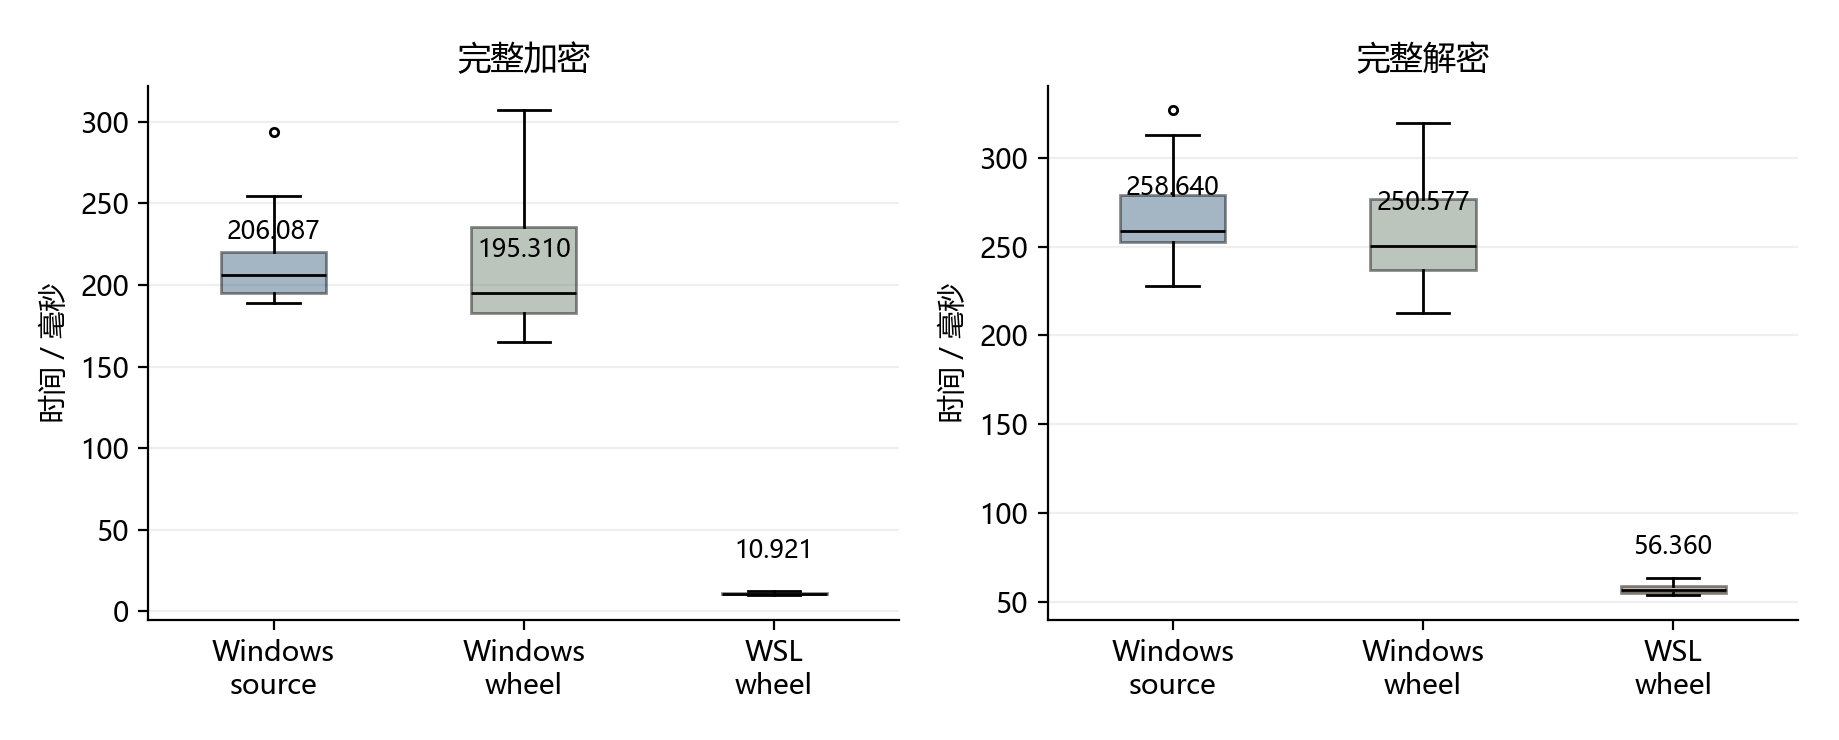
\includegraphics[width=\textwidth,height=0.52\textheight,keepaspectratio]{figures/placement.png}
\caption{同参数完整系统部署消融}\label{fig:placement}
\end{figure}
从同一wheel在两个位置的差异，以及Windows源码与Windows wheel差异较小的结果，可以判断本机主要收益来自运行位置改变。相对Windows源码，WSL副本完整加密与解密约为原来的1/18.87和1/4.59。该实验不降低参数，不减少完整校验，不共享秘密随机性，也不省去wire编解码与原生进程启动。

计时包含公共输入与密钥检查、签验、Hybrid、BYTEAUTH、完整密文编码加载及原生调用。导入、Setup、持久化、恢复和独立计数诊断在热计时之外。每个块的独立诊断中，每对操作均有6次完整源码核对、15次原生调用及5次熵读取，共65644字节。正式批次完整密文范围142036至142153字节，不能替换成前一基线批次的范围。

30次观察共享3套根，不构成30套独立密钥样本。该批内存采用worker进程寿命内核高水位，自身约228.10至229.45MiB，口径不同于上一节的进程树采样；因此不作内存下降结论。该结果也不能外推为其他机器、其他后端或冷启动均有相同提速。

\section{SRGG单体编码实验}
SRGG单体实验使用Core Ultra7 255HX、Sage10.9、Python3.13.15、OMP和OpenBLAS各1线程，与完整系统基线机器不同。三档论文参数均为n=512、p=16383、b=31、w=2、Q=15744063，rank分别2、3、4，采用表格标准差解释。每档3个独立根，共9次生成和18个恢复worker；495项功能检查、54次签名与72次显式验证归档于E07。

\Needspace{11\baselineskip}
\begingroup
\small
\setlength{\tableavail}{\dimexpr\textwidth-6\tabcolsep\relax}
\begin{longtable}{@{}>{\raggedright\arraybackslash}p{0.24\tableavail}>{\raggedright\arraybackslash}p{0.27\tableavail}>{\raggedright\arraybackslash}p{0.25\tableavail}>{\raggedright\arraybackslash}p{0.24\tableavail}@{}}
\caption{SRGG签名无损编码尺寸中位数（单位：字节）}\label{tab:srgg-encoding}\\
\toprule
\rowcolor{black!8} 论文参数档 & 原JSON & compact & 说明 \\
\midrule
\endfirsthead
\multicolumn{4}{l}{\small 表\thetable\quad 续表}\\
\toprule
\rowcolor{black!8} 论文参数档 & 原JSON & compact & 说明 \\
\midrule
\endhead
\midrule
\multicolumn{4}{r}{\small 接下页}\\
\endfoot
\bottomrule
\endlastfoot
PARAM I & 35368 & 13400 & 同一签名对象的两种表示 \\
PARAM II & 51117 & 19288 & 同上 \\
PARAM III & 67076 & 26264 & 同上 \\
\end{longtable}
\endgroup
编码前后没有修改签名方程、采样、参数或默认服务。文件变小带来传输与落盘收益，但完整API可能因编码增加耗时。后续代表B已经把PARAM-I compact与LATTE真实配对，完整密文为149191至149291字节；reference完整密文为171097至171231字节。两批不是同一随机根的配对样本，不能把差值写成计时加速，也不能将单体时间与另一台机器上的完整系统时间排序。

\section{局限与待补实验}
冻结选择时的重复性能收据使用32字节应用消息。E18另补A、B的0／32／1024字节及各自最大应用消息59191／65364字节完整往返，C补0／1024字节；三组容量加1、身份长度加1、格式负例和恢复均通过。主展示另有3根、12组随机身份消息配对的60项检查[E19]。C仍缺3924字节最大消息诚实解密和多根重复，每次解密为分钟级，后续补测设置时间盒。最终发布版本复现和来源许可材料继续收口。

当前用户数还受LATTE两父、每父两子、Sageloli最多两个已发身份等具体profile限制；大规模并发和多写者一致性未在本稿验证。三组安全目标和环境不同，可分别展示成本与用途，但不能仅凭“低通信”“高频”“多用户”标签指定赢家，也不能把C的单根运行冒充重复性能基准。

\chapter{应用展示与技术贡献}
\section{原型使用流程}
网页入口复用公共API，提供LATTE＋ML-DSA、Falcon、Luo三个已验收的交互预设。演示先展示实际算法、参数、身份长度与状态，再由机构生成系统和双方密钥；发送者指定接收身份并加密，接收者指定期望发送身份后解密。随后分别修改发送身份、接收身份和密文字节，观察明确拒绝。页面导出的结果来自实际执行，不使用预填耗时冒充测量。报告代表A可直接用于该流程；B、C通过CLI、冻结配置和预运行收据展示。[E12,E15]

\begin{figure}[htbp]
\centering
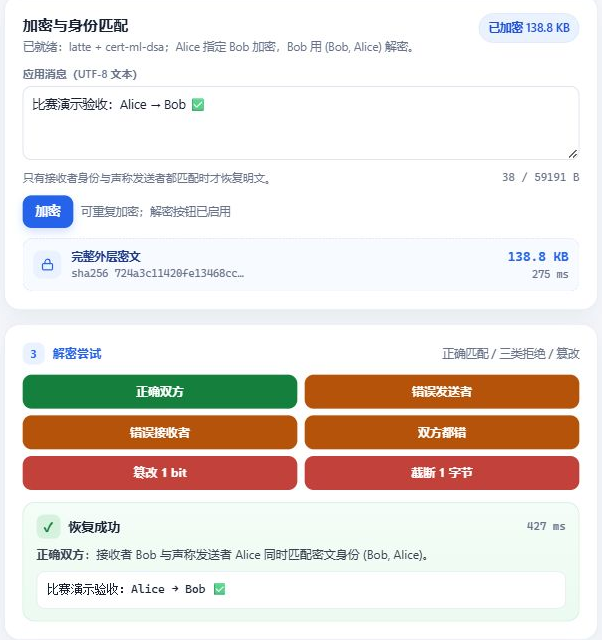
\includegraphics[width=0.82\textwidth,height=0.52\textheight,keepaspectratio]{figures/demo-success-detail.png}
\caption{已归档的合法匹配演示截图局部}\label{fig:demo-success}
\end{figure}
图~\ref{fig:demo-success}从2026年10月18日验收原图裁取加密与合法匹配区域，未改动其中内容，不是本次重新运行截图。截图用于说明应用流程，截图中的单次耗时不替代第5章重复实验。

命令行提供独立持久状态与恢复流程，可在新进程中加载原状态继续解密。网页为单个临时会话，服务重启后需重新建立；这两个入口的状态能力分别解释。网页当前只展示LATTE组合，不能据此宣称所有已登记后端均可在界面任意切换。

\section{模块化实例化贡献}
作品把原语选参、对象编码与公共协议装配分开，使同一双向匹配流程可以复用不同HIBE和IBS。真实结果同时包含LATTE与Lai两种HIBE、认证转换型ML-DSA以及SRGG、Sageloli两种原生IBS。其价值在于把多篇论文方案整理成具有共同契约、容量预检与可核查收据的原型，而不是把算法名称放入一个未实现的下拉框。

支撑材料为公共接口、真实接线验收、三组冻结Suite和完整系统收据。显式provider接口允许新算法在自己的registration模块提供BackendSpec，并原子扩展调用方registry；Suite JSON不能导入代码，stock CLI和Web仍由项目固定清单控制。当前代价包括原生依赖、不同输入上限和运行时差异。该贡献属于系统设计和实现，理论构造按文献署名。

\section{完整流程与状态可靠性贡献}
论文中的一次诚实加解密不直接给出软件重启、重复发钥、配置混用和非规范wire的处理。作品通过规范编码、内部承诺与外部一次性认证、固定身份状态和提交后发布机制，将这些条件形成可检查行为。

对应证据包含四种身份组合、实际完整wire篡改、固定状态加载和新进程零熵恢复。代价是额外密文字段、一次性签名尺寸、持久状态与实现复杂度。相关测试说明实现行为，理论安全依据仍按第2章引用和工作假设解释。

\section{资源与实现优化贡献}
完整系统剖析识别了原生适配器内容校验在跨文件系统访问中的实际成本。保持校验和密码工作后，采用固定wheel的WSL副本取得完整API改进，并通过Windows wheel消融区分“打包”与“位置”两项因素。这一结果具有明确输入、样本组织、版本和计时边界，可按公开工具复核。[E11]

SRGG无损编码与CHKP高基数组件分别提供存储表示和资源可行性方面的研究结果。SRGG PARAM-I compact现已进入代表B；高基数组件及部分CHKP／ABB目标规模仍是独立资源研究。本文保留层级差异，不将编码压缩、部署位置优化和参数投影合并成一个没有测量依据的“联合加速倍数”。

\chapter{总结与后续工作}
本作品已实现两层HIBE与IBS共同装配的IBME框架，并冻结A＝LATTE＋BNN/ML-DSA-44、B＝LATTE＋SRGG PARAM-I compact、C＝Lai C2＋Sageloli RSIS v3 PARAM-I三组报告代表。A具备成熟的Web、安装CLI和重复基准；B展示同一HIBE下原生模块格IBS及无损编码；C展示另一HIBE与环IBS的目标规模完整运行。三组精确profile均按安全方案采用，已知不安全调试档仍被排除。

当前数据同时说明工程代价：A适合现场交互，B的发送发钥和加密更慢，C的密钥、密文和委派开销显著，不适合等待式现场演示。完整系统部署消融还表明，在密码参数不变时消除本机跨文件系统访问热点可以降低热操作耗时；该结论不外推为算法本身加速。

三组精确安装、恢复和内层签名拒绝已完成，A、B最大消息及三组越界已补测；剩余实验为C的3924字节消息和受预算约束的多根重复。随后统一第三方来源许可、本届模板、匿名信息和页数，在同一发布版本复现并检查PDF。ABB、CHKP与Wang目标参数可独立推进，不阻塞三代表报告收口。

\appendix
\chapter{候选路线与实现状态}
\begingroup
\small
\setlength{\tableavail}{\dimexpr\textwidth-4\tabcolsep\relax}
\begin{longtable}{@{}>{\raggedright\arraybackslash}p{0.24\tableavail}>{\raggedright\arraybackslash}p{0.2\tableavail}>{\raggedright\arraybackslash}p{0.56\tableavail}@{}}
\caption{HIBE路线清单}\label{tab:hibe-inventory}\\
\toprule
\rowcolor{black!8} 路线 & 独立完整研究后端 & 截至本稿的状态 \\
\midrule
\endfirsthead
\multicolumn{3}{l}{\small 表\thetable\quad 续表}\\
\toprule
\rowcolor{black!8} 路线 & 独立完整研究后端 & 截至本稿的状态 \\
\midrule
\endhead
\midrule
\multicolumn{3}{r}{\small 接下页}\\
\endfoot
\bottomrule
\endlastfoot
CHKP ROM & 有 & 真实委派和完整接线已有；目标高维另列 \\
ABB ROM & 有 & 可运行研究实例；目标资源与选参另列 \\
LATTE & 有 & seed32／framed32默认安全口径；代表A、B及多组辅助完整运行 \\
GKR2025 & 无 & 暂缓路线 \\
Zhang2020 & 无 & 工具与原稿核验，不是完整后端 \\
ABB标准模型选择性版本 & 无 & 不以ROM版本替代，暂缓 \\
CHKP标准模型版本 & 无 & 不以ROM版本替代，暂缓 \\
Lai理想格HIBE & 有 & C2目标profile默认安全口径；与四种IBS完整配对，代表C采用Sageloli \\
\end{longtable}
\endgroup
\Needspace{30\baselineskip}
\begingroup
\small
\setlength{\tableavail}{\dimexpr\textwidth-4\tabcolsep\relax}
\begin{longtable}{@{}>{\raggedright\arraybackslash}p{0.24\tableavail}>{\raggedright\arraybackslash}p{0.2\tableavail}>{\raggedright\arraybackslash}p{0.56\tableavail}@{}}
\caption{IBS路线清单}\label{tab:ibs-inventory}\\
\toprule
\rowcolor{black!8} 路线 & 独立完整研究后端 & 默认框架与真实接线 \\
\midrule
\endfirsthead
\multicolumn{3}{l}{\small 表\thetable\quad 续表}\\
\toprule
\rowcolor{black!8} 路线 & 独立完整研究后端 & 默认框架与真实接线 \\
\midrule
\endhead
\midrule
\multicolumn{3}{r}{\small 接下页}\\
\endfoot
\bottomrule
\endlastfoot
Luo矩阵版 & 有 & 已登记；研究参数，不恢复不合格参数凑代表 \\
Luo模格版 & 有 & 已登记，LATTE与CHKP接线；默认与C64B分别记录 \\
Wang基本IBS加PW & 有 & 已登记，LATTE接线；q17调试档可公开伪造 \\
SRGG2025 & 有 & 默认小参数与论文参数分ID登记；PARAM-I／II／III默认安全口径，代表B采用PARAM-I compact \\
Yu2026 & 有 & 未默认登记；1至4字节输入不足公共构造 \\
Sageloli SIS & 有 & 未默认登记，未真实HIBE配对 \\
Sageloli RSIS & 有 & 环版v3已登记；PARAM-I／II默认安全口径，已有LATTE桥接与Lai C2代表C[E14,E16] \\
Foo-Li & 有 & 未默认登记，未真实HIBE配对；论文无数值参数，候选目标推导见3.5节与E13 \\
BNN加ML-DSA & 有 & 已登记，多参数LATTE配对；参数档不另计算法 \\
BNN加Falcon & 有 & 已登记，512与1024配对；参数档不另计算法 \\
Xie NTRU IBS & 无 & 修订研究核，尚非共同IBSBackend \\
\end{longtable}
\endgroup
MP12研究变体、高基数参数、编码变化及同算法参数档不另计一篇独立方案。以上状态按当前目录和后续已合入交付共同确定；目录中的旧日期说明保留为历史证据，不能覆盖较新交付。已知不安全调试参数具体记录在E08，不能从某个调试配置的公开伪造推广到整篇论文算法。

\chapter{参数与公开证据索引}
三代表配置、容量和逐组观测以E15的selection.json为当前机器入口；A、B原重复收据和C目标规模收据保持原始Suite摘要，E15同时保存准入更新后的当前摘要与原evidence摘要。图~\ref{fig:legacy-baseline}及旧辅助表来自E04比较JSON，部署消融来自E11，表~\ref{tab:fooli-grid}按明确的q、g和最小\ensuremath{\bar m}从E13逐点结果生成。正文使用归档实测值，文档生成不会调用任何密码采样或打开运行私钥。

\begingroup
\small
\renewcommand{\arraystretch}{1.08}
\setlength{\LTpre}{5pt}
\setlength{\LTpost}{5pt}
\setlength{\tableavail}{\dimexpr\textwidth-4\tabcolsep\relax}
\begin{longtable}{@{}>{\raggedright\arraybackslash}p{0.09\tableavail}>{\raggedright\arraybackslash}p{0.55\tableavail}>{\raggedright\arraybackslash}p{0.36\tableavail}@{}}
\caption{公开证据索引}\label{tab:evidence-index}\\
\toprule
\rowcolor{black!8} 编号 & 证据 & 用途 \\
\midrule
\endfirsthead
\multicolumn{3}{l}{\small 表\thetable\quad 续表}\\
\toprule
\rowcolor{black!8} 编号 & 证据 & 用途 \\
\midrule
\endhead
\midrule
\multicolumn{3}{r}{\small 接下页}\\
\endfoot
\bottomrule
\endlastfoot
E01 & \evidenceitem{MLDSA完整基线}{docs/research/2026-10-18-full-system-baseline/README.md} & 版本输入计时尺寸与恢复 \\
E02 & \evidenceitem{Falcon完整基线}{docs/research/2026-10-18-full-system-falcon/README.md} & 同上 \\
E03 & \evidenceitem{Luo完整基线}{docs/research/2026-10-18-full-system-luo/README.md} & 同上 \\
E04 & \evidenceitem{三组参数卡}{docs/deliveries/2026-10-18-main-showcase-cards/README.md}\evidenceitem{比较JSON}{docs/research/2026-10-18-full-system-luo/evidence/comparison.json} & 三组Suite参数和统一统计 \\
E05 & \evidenceitem{IBS接入盘点与C64B}{docs/deliveries/2026-10-18-ibs-inventory/README.md} & 实际默认入口与C64B完整运行 \\
E06 & \evidenceitem{共同框架真实接入}{docs/research/team-c-delivery/2026-10-15-c-framework/README.md}\evidenceitem{CHKP及Luo}{docs/deliveries/2026-10-12-chkp-luo/README.md} & 真实配对与CLI边界 \\
E07 & \evidenceitem{SRGG compact与论文参数基准}{docs/research/team-b-delivery/2026-10-18-srgg-compact-benchmark/README_zh-CN.md} & 单体采样签验恢复与编码 \\
E08 & \evidenceitem{算法总表}{docs/ALGORITHM_CATALOG.md} & 19条路线和各独立交付入口 \\
E09 & \evidenceitem{高基数有界运行}{docs/research/team-a-delivery/2026-10-18-bounded-radix/README.md}\evidenceitem{组件接收}{docs/deliveries/2026-10-18-pr43-48-review/README.md} & 小规模组件与目标投影 \\
E10 & \evidenceitem{ABB紧边界资源材料}{docs/research/team-a-delivery/2026-10-18-abb-tight-frontier/README.md} & 公开参数算术与资源下界 \\
E11 & \evidenceitem{完整系统运行位置消融}{docs/research/2026-10-19-full-system-placement/README.md} & 三路完整计时与版本校验 \\
E12 & \evidenceitem{演示实际验收}{docs/deliveries/2026-10-18-demo-acceptance/README.md}\evidenceitem{后续审查}{docs/deliveries/2026-10-19-pr-review/README.md} & Web与CLI及判定修订 \\
E13 & \evidenceitem{Foo-Li参数改进搜索与逐点结果}{docs/research/2026-10-19-parameters/fooli-improvement-search.json} & 有限网格预筛、模型估计与候选目标卡 \\
E14 & \evidenceitem{Sageloli环版论文参数实跑}{docs/research/team-b-delivery/2026-10-19-sageloli-ring-target/README_zh-CN.md} & 论文两点独立实跑与边界 \\
E15 & \evidenceitem{三代表选择、冻结Suite与机器记录}{docs/deliveries/2026-10-19-report-three-selection/README.md} & A／B／C参数、容量、摘要、观测及剩余验收 \\
E16 & \evidenceitem{Lai C2四组合完整收据}{docs/research/2026-10-19-lai-c2-combinations/README.md}\evidenceitem{Sageloli公共接入}{docs/research/2026-10-19-sageloli-ring-integration/README.md} & C的目标规模完整运行与LATTE桥接 \\
E17 & \evidenceitem{已完成方案安全前提}{docs/deliveries/2026-10-19-project-admission/README.md} & 已完成默认安全与已知反例单列 \\
E18 & \evidenceitem{同机实验主表与安装补测}{docs/deliveries/2026-10-19-report-experiment-supplement/README.md} & A／B各三根，三组64条CLI与3个内层负例 \\
E19 & \evidenceitem{主展示随机批量验收}{docs/research/2026-10-19-primary-random-batch/README.md} & 独立Xeon环境3根、12配对、60项检查 \\
\end{longtable}
\endgroup


\section*{同机A/B补充基准}
本表来自E18的独立同机批次，单位为秒、中位数。每组3个独立CSPRNG根、9对热运行与9次恢复后解密；消息32字节、身份64字节，同一源码wheel与i9-14900HX／Sage10.7环境，OMP4／BLAS1。不同操作的样本数量、根间依赖及逐次数据见原公开主表，不作等安全排名。
\begingroup
\small
\setlength{\tableavail}{\dimexpr\textwidth-4\tabcolsep\relax}
\begin{longtable}{@{}>{\raggedright\arraybackslash}p{0.44\tableavail}>{\raggedright\arraybackslash}p{0.28\tableavail}>{\raggedright\arraybackslash}p{0.28\tableavail}@{}}
\caption{同机A/B完整系统补充基准}\label{tab:same-machine-ab}\\
\toprule
\rowcolor{black!8} 操作 & A：LATTE＋BNN/ML-DSA & B：LATTE＋SRGG \\
\midrule
\endfirsthead
\multicolumn{3}{l}{\small 表\thetable\quad 续表}\\
\toprule
\rowcolor{black!8} 操作 & A：LATTE＋BNN/ML-DSA & B：LATTE＋SRGG \\
\midrule
\endhead
\midrule
\multicolumn{3}{r}{\small 接下页}\\
\endfoot
\bottomrule
\endlastfoot
Setup & 1.117252 & 1.598913 \\
发送者发钥 & 0.095386 & 32.066890 \\
接收者发钥 & 0.426875 & 0.456980 \\
首次加密 & 0.096330 & 9.142216 \\
首次解密（含叶生成） & 0.283574 & 0.238744 \\
热加密 & 0.078473 & 9.172154 \\
热解密 & 0.151951 & 0.160670 \\
新进程对象恢复 & 0.844533 & 0.889801 \\
恢复后解密 & 0.153717 & 0.133632 \\
\end{longtable}
\endgroup
E18另外完成64条精确安装CLI及3个完整协议内层负例。每个应用长度只有一次同根观察，不能与重复基准混计。C只测0和1024字节，四次解密均执行真实未缓存委派。原临时私有状态未能归档的限制见E18；公开收据及源码保持原值，不将历史恢复成功写成可移交原状态。

\chapter*{参考文献}
\addcontentsline{toc}{chapter}{参考文献}
\begingroup
\footnotesize
\linespread{1.04}\selectfont
\let\small\footnotesize
\raggedright
\setlength{\parskip}{1pt}
\begingroup\small\noindent [1] Yuejun Wang, Baocang Wang, Qiqi Lai, Yu Zhan. Identity-based Matchmaking Encryption with Stronger Security and Instantiation on Lattices. Theoretical Computer Science. DOI 10.1016/j.tcs.2024.115048. 固定本地稿见 \nolinkurl{papers/2022_identity_matchmaking_wang.pdf}，Construction 1及相关图表。\par\endgroup

\begingroup\small\noindent [2] David Cash, Dennis Hofheinz, Eike Kiltz, Chris Peikert. Bonsai Trees, or How to Delegate a Lattice Basis. EUROCRYPT 2010，固定作者全文2011年6月14日版，\S{}5。\par\endgroup

\begingroup\small\noindent [3] Shweta Agrawal, Dan Boneh, Xavier Boyen. Efficient Lattice (H)IBE in the Standard Model. 2010，固定40页作者全文，\S{}7与\S{}8的结论范围分别使用。\par\endgroup

\begingroup\small\noindent [4] Raymond K. Zhao, Sarah McCarthy, Ron Steinfeld, Amin Sakzad, Máire O'Neill. Quantum-safe HIBE: does it cost a LATTE? IEEE Transactions on Information Forensics and Security，固定作者接受稿。\par\endgroup

\begingroup\small\noindent [5] Pingbin Luo, Xinjian Chen, Willy Susilo, Qiong Huang. Identity-Based Signature from Lattices without Trapdoors. ICICS 2024，\S{}3与\S{}4。\par\endgroup

\begingroup\small\noindent [6] Huiwen Jia, Ying Liu, Chunming Tang, Lin Wang. Constructing Efficient Identity-Based Signatures on Lattices. IET Information Security, 2025. DOI 10.1049/ise2/6684889.\par\endgroup

\begingroup\small\noindent [7] Jiaxin Pan, Benedikt Wagner. Short Identity-Based Signatures with Tight Security from Lattices. PQCrypto 2021. DOI 10.1007/978-3-030-81293-5\_19.\par\endgroup

\begingroup\small\noindent [8] Ernest Foo, Qinyi Li. Tightly Secure Lattice Identity-Based Signature in the Quantum Random Oracle Model. ACISP 2023. DOI 10.1007/978-3-031-35486-1\_17.\par\endgroup

\begingroup\small\noindent [9] Qing Yu, Shengli Liu, Yiming Li. Identity-based signature and identity-based matchmaking encryption from lattices. Theoretical Computer Science, 2026. DOI 10.1016/j.tcs.2026.116152.\par\endgroup

\begingroup\small\noindent [10] Éric Sageloli, Pierre Pébereau, Pierrick Méaux, Céline Chevalier. Shorter and Faster Identity-Based Signatures with Tight Security in the (Q)ROM from Lattices. ACNS 2023. DOI 10.1007/978-3-031-33488-7\_24. 使用HAL73页完整稿，\S{}5至\S{}8及附录E。\par\endgroup

\begingroup\small\noindent [11] David Galindo, Javier Herranz, Eike Kiltz. On the Generic Construction of Identity-Based Signatures with Additional Properties. ASIACRYPT 2006，\S{}3与Theorem 1。本文据此引用认证转换的重述，不将其列为本作品原创。\par\endgroup

\begingroup\small\noindent [12] NIST. Module-Lattice-Based Digital Signature Standard. FIPS 204, 2024. 固定本地官方PDF与底层参数表。\par\endgroup

\begingroup\small\noindent [13] Pierre-Alain Fouque 等. Falcon Fast-Fourier Lattice-based Compact Signatures over NTRU. Specification v1.2, 2020.\par\endgroup

\begingroup\small\noindent [14] Daniele Micciancio, Chris Peikert. Trapdoors for Lattices Simpler Tighter Faster Smaller. EUROCRYPT 2012，固定本地2011年9月14日作者稿。\par\endgroup

\begingroup\small\noindent [15] Russell W. F. Lai, Henry K. F. Cheung, Sherman S. M. Chow. Trapdoors for Ideal Lattices with Applications. Inscrypt 2014, LNCS 8957:239--256, 2015. DOI 10.1007/978-3-319-16745-9\_14. 本文使用本地归档的完整PDF及\S{}5.1--5.2与Theorem 10。\par\endgroup

以上文献的归档版本与文件指纹以支撑材料中的\nolinkurl{papers/index.md}为准。正式成稿还需统一文献格式并完成第三方代码与许可证清单；当前引用不替代该清单。
\par\endgroup

\end{document}
